\documentclass{article}
% Problems transcribed from Problem Set 4.pdf; the missing square in Problem 1(a) was corrected.
% The TikZ redrawings, upright textual subscripts, and minimal mathematical corrections were prepared with AI assistance.
\usepackage[en]{homework}
\usepackage{tikz}

\config{Physics-1}{2026 Fall}{4}

\begin{document}

\begin{problem}
\begin{enumerate}
  \item[a)] The spherical polar coordinates are defined as follows:
  \[
    z=r\cos\theta,\quad y=r\sin\theta\sin\phi,\qquad x=r\sin\theta\cos\phi
  \]
  \begin{center}
    \resizebox{0.42\linewidth}{!}{% AI-assisted TikZ reconstruction of the source spherical-coordinate diagram.
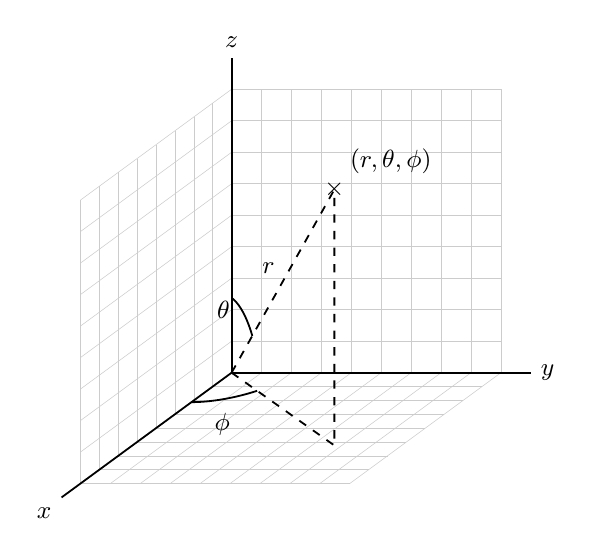
\begin{tikzpicture}[
  x={(-0.60cm,-0.44cm)}, y={(0.95cm,0cm)}, z={(0cm,1cm)},
  line width=0.65pt, font=\small
]
  % The three coordinate planes have transparent backgrounds.
  \foreach \a in {0,0.4,...,3.2} {
    \draw[gray!40,line width=0.2pt] (\a,0,0) -- (\a,3.6,0);
    \draw[gray!40,line width=0.2pt] (\a,0,0) -- (\a,0,3.6);
  }
  \foreach \b in {0,0.4,...,3.6} {
    \draw[gray!40,line width=0.2pt] (0,\b,0) -- (3.2,\b,0);
    \draw[gray!40,line width=0.2pt] (0,\b,0) -- (0,\b,3.6);
    \draw[gray!40,line width=0.2pt] (0,0,\b) -- (3.2,0,\b);
    \draw[gray!40,line width=0.2pt] (0,0,\b) -- (0,3.6,\b);
  }
  \coordinate (O) at (0,0,0);
  \coordinate (P) at (2.1,2.7,3.25);
  \coordinate (Q) at (2.1,2.7,0);
  \draw (O) -- (3.6,0,0) node[below left] {$x$};
  \draw (O) -- (0,4.0,0) node[right] {$y$};
  \draw (O) -- (0,0,4.0) node[above] {$z$};
  \draw[dashed] (O) -- (P) node[pos=0.57,left=2pt] {$r$};
  \draw[dashed] (O) -- (Q) -- (P);
  \node[inner sep=0pt] at (P) {$\times$};
  \node[above right=2pt] at (P) {$(r,\theta,\phi)$};
  \draw plot[domain=0:46.55,samples=28,variable=\t]
    ({0.95*sin(\t)*cos(52.13)},
     {0.95*sin(\t)*sin(52.13)},{0.95*cos(\t)});
  \node[left] at (0.17,0.22,0.87) {$\theta$};
  \draw plot[domain=0:52.13,samples=28,variable=\t]
    ({0.85*cos(\t)},{0.85*sin(\t)},0);
  \node[below] at ({0.98*cos(26)},{0.98*sin(26)},0) {$\phi$};
\end{tikzpicture}
}\quad
    \resizebox{0.46\linewidth}{!}{% AI-assisted TikZ reconstruction of the source spherical surface element.
\begin{tikzpicture}[
  x={(-0.60cm,-0.44cm)}, y={(0.95cm,0cm)}, z={(0cm,1cm)},
  line width=0.65pt, font=\small, >=stealth
]
  \def\Rad{3.3}
  \def\ThetaA{43}
  \def\ThetaB{55}
  \def\PhiA{52}
  \def\PhiB{69}
  \coordinate (O) at (0,0,0);
  \coordinate (Paa) at
    ({\Rad*sin(\ThetaA)*cos(\PhiA)},
     {\Rad*sin(\ThetaA)*sin(\PhiA)},{\Rad*cos(\ThetaA)});
  \coordinate (Pab) at
    ({\Rad*sin(\ThetaA)*cos(\PhiB)},
     {\Rad*sin(\ThetaA)*sin(\PhiB)},{\Rad*cos(\ThetaA)});
  \coordinate (Pba) at
    ({\Rad*sin(\ThetaB)*cos(\PhiA)},
     {\Rad*sin(\ThetaB)*sin(\PhiA)},{\Rad*cos(\ThetaB)});
  \coordinate (Pbb) at
    ({\Rad*sin(\ThetaB)*cos(\PhiB)},
     {\Rad*sin(\ThetaB)*sin(\PhiB)},{\Rad*cos(\ThetaB)});
  \coordinate (Qba) at
    ({\Rad*sin(\ThetaB)*cos(\PhiA)},
     {\Rad*sin(\ThetaB)*sin(\PhiA)},0);
  \coordinate (Qbb) at
    ({\Rad*sin(\ThetaB)*cos(\PhiB)},
     {\Rad*sin(\ThetaB)*sin(\PhiB)},0);
  \draw[->,gray!80] (O) -- (3.65,0,0) node[below left,black] {$x$};
  \draw[->,gray!80] (O) -- (0,3.75,0) node[right,black] {$y$};
  \draw[->,gray!80] (O) -- (0,0,3.75) node[above,black] {$z$};
  % Visible spherical octant and a meridian/latitude through the patch.
  \draw[blue!45] plot[domain=0:90,samples=50,variable=\t]
    ({\Rad*sin(\t)},0,{\Rad*cos(\t)});
  \draw[blue!45] plot[domain=0:90,samples=50,variable=\t]
    (0,{\Rad*sin(\t)},{\Rad*cos(\t)});
  \draw[blue!45] plot[domain=0:90,samples=50,variable=\t]
    ({\Rad*cos(\t)},{\Rad*sin(\t)},0);
  \draw[gray,densely dotted] plot[domain=0:90,samples=50,variable=\t]
    ({\Rad*sin(\t)*cos(\PhiA)},
     {\Rad*sin(\t)*sin(\PhiA)},{\Rad*cos(\t)});
  \draw[gray] plot[domain=0:90,samples=50,variable=\t]
    ({\Rad*sin(\ThetaA)*cos(\t)},
     {\Rad*sin(\ThetaA)*sin(\t)},{\Rad*cos(\ThetaA)});
  \draw[gray,dashed] (Pba) -- (Qba) -- (O) -- (Qbb) -- (Pbb);
  \draw[gray] (O) -- (Paa) node[pos=0.48,right,text=black] {$r$};
  \draw[gray] (O) -- (Pba);
  \draw[gray] (0,0,{\Rad*cos(\ThetaA)}) -- (Paa)
    node[midway,above,sloped,text=black] {$r\sin\theta$};
  % Curved boundaries follow the two meridians and two latitudes.
  \path[fill=cyan!30,draw=blue!60!black]
    plot[domain=\PhiA:\PhiB,samples=16,variable=\t]
      ({\Rad*sin(\ThetaA)*cos(\t)},
       {\Rad*sin(\ThetaA)*sin(\t)},{\Rad*cos(\ThetaA)})
    -- plot[domain=\ThetaA:\ThetaB,samples=16,variable=\t]
      ({\Rad*sin(\t)*cos(\PhiB)},
       {\Rad*sin(\t)*sin(\PhiB)},{\Rad*cos(\t)})
    -- plot[domain=\PhiB:\PhiA,samples=16,variable=\t]
      ({\Rad*sin(\ThetaB)*cos(\t)},
       {\Rad*sin(\ThetaB)*sin(\t)},{\Rad*cos(\ThetaB)})
    -- plot[domain=\ThetaB:\ThetaA,samples=16,variable=\t]
      ({\Rad*sin(\t)*cos(\PhiA)},
       {\Rad*sin(\t)*sin(\PhiA)},{\Rad*cos(\t)}) -- cycle;
  \node at
    ({\Rad*sin(49)*cos(60.5)},
     {\Rad*sin(49)*sin(60.5)},{\Rad*cos(49)}) {$\mathrm{d}A$};
  \draw[gray,->] plot[domain=0:\ThetaA,samples=30,variable=\t]
    ({0.75*sin(\t)*cos(\PhiA)},
     {0.75*sin(\t)*sin(\PhiA)},{0.75*cos(\t)});
  \node[left] at (0.12,0.15,0.68) {$\theta$};
  \draw[gray,->] plot[domain=\ThetaA:\ThetaB,samples=15,variable=\t]
    ({1.25*sin(\t)*cos(\PhiA)},
     {1.25*sin(\t)*sin(\PhiA)},{1.25*cos(\t)});
  \coordinate (AngleDtheta) at
    ({1.25*sin(49)*cos(\PhiA)},
     {1.25*sin(49)*sin(\PhiA)},{1.25*cos(49)});
  \draw[gray] (AngleDtheta) -- ([xshift=0.35cm,yshift=-0.15cm]AngleDtheta);
  \node[right,inner sep=1pt,fill=shadecolor] at
    ([xshift=0.35cm,yshift=-0.15cm]AngleDtheta) {$\mathrm{d}\theta$};
  \draw[gray,->] plot[domain=0:\PhiA,samples=30,variable=\t]
    ({0.82*cos(\t)},{0.82*sin(\t)},0);
  \node[below] at ({0.95*cos(26)},{0.95*sin(26)},0) {$\phi$};
  \draw[gray,->] plot[domain=\PhiA:\PhiB,samples=16,variable=\t]
    ({1.85*cos(\t)},{1.85*sin(\t)},0);
  \node[below,inner sep=1pt,fill=shadecolor] at
    ({1.85*cos(60.5)},{1.85*sin(60.5)},0) {$\mathrm{d}\phi$};
  % Red dimension brackets retain the labels in the source drawing.
  \draw[red!65!black] (Pab) -- ([xshift=0.17cm]Pab)
    -- ([xshift=0.17cm]Pbb) -- (Pbb);
  \path (Pab) -- (Pbb) coordinate[midway] (Dtheta);
  \draw[red!65!black] ([xshift=0.17cm]Dtheta)
    -- ([xshift=0.65cm,yshift=0.35cm]Dtheta)
    -- ([xshift=1.8cm,yshift=0.35cm]Dtheta)
    node[right,black] {$r\,\mathrm{d}\theta$};
  \draw[red!65!black] (Pba) -- ([yshift=-0.16cm]Pba)
    -- ([yshift=-0.16cm]Pbb) -- (Pbb);
  \path (Pba) -- (Pbb) coordinate[midway] (Dphi);
  \draw[red!65!black] ([yshift=-0.16cm]Dphi)
    -- ([xshift=0.35cm,yshift=-0.45cm]Dphi)
    -- ([xshift=2.0cm,yshift=-0.45cm]Dphi)
    node[right,black] {$r\sin\theta\,\mathrm{d}\phi$};
\end{tikzpicture}
}
  \end{center}
  From the picture, compute the area of the infinitesimal blue rectangle at the surface of the sphere at radius $r$.

  Consider a spherical shell with mass/Area $=\rho$ and radius $R$.
  Compute the moment of inertia of this shell when the rotation axis goes through the center of the shell. (let's say along the $z$-axis)
  (The moment of inertia of a particle from a rotation axis is given by mass $\times$ the square of the perpendicular distance from the rotation axis. One therefore has to integrate over the contribution of every part on the surface of the sphere)
  Express the final answer in terms of the total mass and the radius $R$.

  \item[b)] Now instead we have a solid ball of radius $R$ and it has density (mass/volume) $\rho$.
  Compute the moment of inertia for the ball when the rotation axis is also going through the center of the ball.
  If the ball and the shell in (a) has the same mass, which one has a bigger moment of inertia?
  \item[c)] Compute the moment of inertia of a cylinder of radius $r$ and height $h$ for a rotation axis passing through the central axis of the cylinder.
\end{enumerate}
\end{problem}

\begin{solution}
	\paragraph{(a)} It's known that $\d A = r^2 \sin \theta \d \theta \d \phi$. The moment of inertia is calculated by definition: 
	\[ I = \int_{}^{}r_\perp^2 \d m 
	= \int_{\theta = 0}^{\pi} \int_{\phi = 0}^{2\pi} (R \sin \theta)^2 \rho R^2 \sin \theta \d \phi \d \theta = \frac{2mR^2}{3}. \]

	\paragraph{(b)} 
	\[ I' = \int_{r = 0}^{R} \int_{\theta = 0}^{\pi} \int_{\phi = 0}^{2\pi} (r \sin \theta)^2 \rho r^2 \sin \theta \d \phi \d \theta \d r = \frac{2mR^2}{5} \]
	In fact, $I' < I$, since the mass distributes closer to the center of mass in a solid sphere than a shell. 

	\paragraph{(c)} For a uniform solid cylinder, let $s$ denote the distance from its axis. Then
	\[ I = \int_0^r s^2 \frac{m}{\pi r^2h} 2\pi s h \d s = \frac{1}{2}mr^2. \]
\end{solution}



\begin{problem}
\begin{enumerate}
  \item[a)] Suppose a body of mass $m$ is rotated about an axis $z$ passing through the body's center of mass. The parallel axis theorem states that if the body is made to rotate instead about a new axis $z'$, which is parallel to the first axis and displaced from it by a distance $d$, then the moment of inertia $I$ with respect to the new axis is related to $I_{\mathrm{cm}}$ by
  \[
    I=I_{\mathrm{cm}}+md^2
  \]
  Prove this statement.
  \begin{center}
    \resizebox{!}{4.1cm}{% AI-assisted TikZ reconstruction of the source parallel-axis diagram.
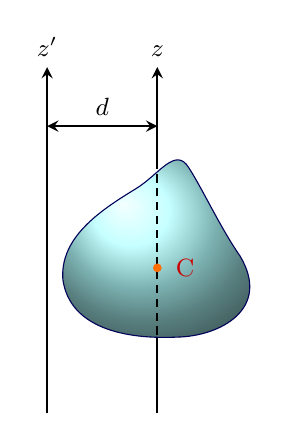
\begin{tikzpicture}[line width=0.8pt,>=stealth,font=\small]
  \draw[->,thick] (0,0) -- (0,4.4) node[above] {$z'$};
  \draw[thick] (1.4,0) -- (1.4,1.0);
  \shade[ball color=cyan!30,draw=blue!35!black,line width=0.4pt]
    (0.2,1.7)
    .. controls (0.16,2.23) and (0.66,2.57) .. (1.12,2.85)
    .. controls (1.42,3.03) and (1.63,3.4) .. (1.8,3.12)
    .. controls (1.98,2.84) and (2.2,2.36) .. (2.45,2.0)
    .. controls (2.85,1.33) and (2.2,0.98) .. (1.65,0.97)
    .. controls (1.0,0.94) and (0.29,1.08) .. (0.2,1.7) -- cycle;
  \draw[thick,densely dashed] (1.4,1.0) -- (1.4,3.12);
  \draw[->,thick] (1.4,3.12) -- (1.4,4.4) node[above] {$z$};
  \draw[<->] (0,3.65) -- (1.4,3.65) node[midway,above] {$d$};
  \fill[orange!85!red] (1.4,1.85) circle (0.055);
  \node[right=3pt,text=red!80!black] at (1.4,1.85) {$\mathrm C$};
\end{tikzpicture}
}
  \end{center}
  \item[b)] Prove the perpendicular-axis theorem: for planar (i.e. 2D) objects lying in the $x$-$y$ plane, the moments of inertia $I_x$, $I_y$, $I_z$ around the $x$-, $y$-, $z$-axis, respectively, are related by $I_z=I_x+I_y$.
\end{enumerate}
\end{problem}

\begin{solution}
	\paragraph{(a)} Distinguish the distance from $z$ and $z'$ by index $z$ and $z'$. Select the origin point as the center of mass, and let $\bo{d}$ be the vector perpendicular to $z$-axis, pointing to $z'$-axis. From the geometric relation, given a point $\bo{r}$, we have
	\[ d_{z}^2 = (\bo{r} - (\bo{r} \cdot \hat{\bo{z}})\hat{\bo{z}})^2, \quad 
	d_{z'}^2 = (\bo{r} - (\bo{r} \cdot \hat{\bo{z}})\hat{\bo{z}} - \bo{d})^2. \]
	Therefore, using $\int_{}^{}\bo{r}\d m = 0$, we can calculate $I$ as
	\begin{align*}
		I
		&= \int_{}^{}d_{z'}^2 \d m 
		= \int_{}^{}(\bo{r} - (\bo{r} \cdot \hat{\bo{z}})\hat{\bo{z}} - \bo{d})^2\d m \\
		&= \int_{}^{} \left\{ (\bo{r} - (\bo{r} \cdot \hat{\bo{z}})\hat{\bo{z}})^2 + d^2 - 2 \bo{d} \cdot (\bo{r} - (\bo{r} \cdot \hat{\bo{z}})\hat{\bo{z}}) \right\} \d m \\
		&= \int_{}^{}d_{z}^2 \d m + md^2 - 2 \bo{d} \cdot \int_{}^{}\bo{r} \d m + 2\int_{}^{}(\bo{r} \cdot \hat{\bo{z}}) (\hat{\bo{z}} \cdot \bo{d}) \d m \\
		&= I_{\mathrm{cm}} + md^2.
	\end{align*}

	\paragraph{(b)} From the geometric relation, for any point in $x$ - $y$ plane, $d_z^2 = d_x^2 + d_y^2$, then the result follows as
	\[ I_z = \int_{}^{}d_z^2 \d m = \int_{}^{} (d_x^2 + d_y^2) \d m = I_x + I_y. \]
\end{solution}



\begin{problem}
Consider an object with mass $M$ that is both translating and rotating. The angular velocity is $\omega$, and the velocity of the center of mass (CM) is $\overrightarrow{v_{\mathrm{cm}}}$. The position of the CM at the instant shown, with respect to the origin is $\overrightarrow{r_{\mathrm{cm}}}$. Show that the total angular momentum of this object, relative to the origin, is given by
\[
  \overrightarrow{L_{\mathrm{total}}}=M\,\overrightarrow{r_{\mathrm{cm}}}\times\overrightarrow{v_{\mathrm{cm}}}+\overrightarrow{L_{\mathrm{around\ CM}}}.
\]
\end{problem}

\begin{proof}
	Let the vector of angular velocity be $\bo{\omega}$. For a point on the rigid body of position $\bo{r}$ with respect to the origin point, its velocity is given by
	\[ \bo{v} = \bo{v}_{\mathrm{cm}} + \bo{\omega} \times (\bo{r} - \bo{r}_{\mathrm{cm}}). \]
	Therefore,
	\begin{align*}
		\bo{L}_{\mathrm{total}}
		&= \int_{}^{}\bo{r} \times \bo{v} \d m \\
		&= \int_{}^{}\left\{ (\bo{r}_{\mathrm{cm}} + (\bo{r} - \bo{r}_{\mathrm{cm}})) \times (\bo{v}_{\mathrm{cm}} + \bo{\omega} \times (\bo{r} - \bo{r}_{\mathrm{cm}})) \right\}\d m \\
		&= (\bo{r}_{\mathrm{cm}} \times \bo{v}_{\mathrm{cm}}) \int_{}^{}\d m 
		+ \bo{r}_{\mathrm{cm}} \times \left( \bo{\omega} \times \int_{}^{}(\bo{r} - \bo{r}_{\mathrm{cm}}) \d m \right) \\
		&\quad + \left( \int_{}^{}(\bo{r} - \bo{r}_{\mathrm{cm}}) \d m \right) \times \bo{v}_{\mathrm{cm}} 
		+ \int_{}^{}(\bo{r} - \bo{r}_{\mathrm{cm}}) \times (\bo{v} - \bo{v}_{\mathrm{cm}}) \d m \\
		&= M \bo{r}_{\mathrm{cm}} \times \bo{v}_\mathrm{cm} + \bo{L}_{\mathrm{around\ CM}}. 
	\end{align*}
\end{proof}



\begin{problem}
Consider two objects with $m_1>m_2$ connected by a light string that passes over a pulley having a moment of inertia of $I$ about its axis of rotation as shown in the the figure below. The string does not slip on the pulley or stretch. The pulley turns without friction. The two objects are released from rest separated by a vertical distance $2h$.
\begin{enumerate}
  \item[a)] Use the principle of conservation of energy to find the translational speeds of the objects as they pass each other.
  \item[b)] Find the angular speed of the pulley at this time.
\end{enumerate}
\begin{center}
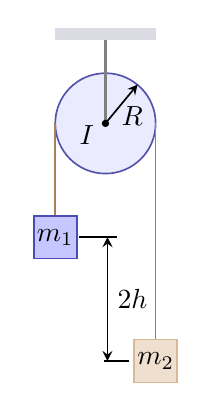
\begin{tikzpicture}[scale=0.85, line width=0.6pt, >=stealth]
  \fill[blue!12!gray!25] (-0.75,3.35) rectangle (0.75,3.53);
  \draw[gray] (0,3.35) -- (0,2.85);
  \draw[draw=blue!35!gray, fill=blue!8] (0,2.1) circle (0.75);
  \draw[gray, thick] (0,3.35) -- (0,2.1);
  \fill (0,2.1) circle (0.055);
  \draw[->] (0,2.1) -- (0.48,2.68);
  \node at (0.40,2.21) {$R$};
  \node at (-0.28,1.92) {$I$};
  \draw[brown!65!gray] (-0.75,2.1) -- (-0.75,0.72);
  \draw[brown!65!gray] (0.75,2.1) -- (0.75,-1.13);
  \draw[draw=blue!40!gray, fill=blue!22] (-1.07,0.08) rectangle (-0.43,0.72);
  \node at (-0.75,0.4) {$m_1$};
  \draw[draw=brown!55, fill=brown!25] (0.43,-1.77) rectangle (1.07,-1.13);
  \node at (0.75,-1.45) {$m_2$};
  \draw (-0.4,0.4) -- (0.17,0.4);
  \draw (0.35,-1.45) -- (-0.02,-1.45);
  \draw[<->] (0.03,0.4) -- (0.03,-1.45) node[midway,right] {$2h$};
\end{tikzpicture}
\end{center}
\end{problem}

\begin{solution}
	\paragraph{(a)} Suppose the translation speeds are both $v$. Since the string does not slip, the angular velocity of the pulley is $v/R$, and hence the kinetic energy of the system is
	\[ \frac{1}{2}(m_1 + m_2)v^2 + \frac{1}{2} I \left( \frac{v}{R} \right)^2. \]

	The kinetic energy comes from the loss of the potential of the gravity $(m_1 - m_2)gh$. Therefore, we got
	\[ v = \sqrt{\frac{2gh(m_1 - m_2)}{m_1 + m_2 + I/R^2}} \]

	\paragraph{(b)} 
	\[ \omega = \frac{v}{R} = \sqrt{\frac{2gh(m_1 - m_2)}{R^2(m_1 + m_2) + I}}. \]
\end{solution}



\begin{problem}
(optional) Let us go back to the problem where we claim generally the angular velocity $\vec\omega$ is not parallel to angular momentum $\vec L$.

The angular momentum of a rigid object can be calculated by
\[
  L=\int\vec r\times(dm\,\vec v)
\]
Where $dm$ is an infinitesimal mass element of the object and the integral is performed over the volume of the object.
\begin{enumerate}
  \item[a)] Using the relation $\vec v=\vec\omega\times\vec r$ between the velocity and angular velocity vectors, show that $\vec L=I\vec\omega$, where $I$ is a $3\times3$ matrix with components
  \begin{gather*}
    I_{xx}=\int dm\,(y^2+z^2),\quad I_{yy}=\int dm\,(z^2+x^2),\quad I_{zz}=\int dm\,(y^2+x^2) \\
    I_{xy}=I_{yx}=-\int dm\,(xy),\quad I_{yz}=I_{zy}=-\int dm\,(yz),\quad I_{zx}=I_{xz}=-\int dm\,(zx)
  \end{gather*}
  \item[b)] Show that for a two-dimensional (``thin'') object lying in the $xy$ plane and rotating around the $z$-axis with angular velocity $\vec\omega=\omega\vec k$, the angular momentum is given by $\vec L=I_{zz}\,\omega\vec k$.
\end{enumerate}
\end{problem}

\begin{solution}
	\paragraph{(a)} We use Einstein's Summation notation in the following calculation.
	\begin{align*}
		L_i &= \int_{}^{}(\bo{r} \times \bo{v})_i\d m
		= \int_{}^{}\varepsilon_{ijk}r_j (\bo{\omega} \times \bo{r})_k \d m \\
		&= \int_{}^{}\varepsilon_{ijk}\varepsilon_{klm}r_j \omega_l r_m \d m \\
		&= \int_{}^{}(\delta_{il} \delta_{jm} - \delta_{im} \delta_{jl})r_j r_m \omega_l \d m \\
		&= \left( \int_{}^{} (\delta_{ij} r^2 - r_i r_j)\d m \right) \omega_j,
	\end{align*}
	where $\int_{}^{} (\delta_{ij} r^2 - r_i r_j)\d m$ is equal to the given matrix.

	\paragraph{(b)} In the case of a thin object lying in the $xy$ plane, $z=0$ everywhere, and therefore $I_{zz} = I_{xx} + I_{yy}$, $I_{xz} = I_{yz} = 0$. Since $\bo{\omega} = \omega \hat{\bo{z}}$, we have
	\[ \bo{L} = \omega\left( I_{xz} \hat{\bo{x}} + I_{yz} \hat{\bo{y}} + I_{zz} \hat{\bo{z}} \right) = I_{zz} \omega \hat{\bo{z}}. \]
\end{solution}

\end{document}
